% % % % % % % % % % % % % % % % % % % % % % % % % % % % % % % % % % % % % % % %
% IEEE Style - Double columns, 11pt font, letterpaper
\documentclass[journal, twocolumn, final,11pt,letterpaper]{IEEEtran}	

% Include Latex Packages
\usepackage{etex}	% This package enables the use of many packages

% % Page styles
\usepackage{setspace}	% line spacing package
\doublespacing			% use double spacing
%\linespread{1.6}		% Use linespread to fine tune line spacing, not recommended


% % Figures
\usepackage{float}		% improves interface for floating objects
\usepackage{subfig}		% enables subfloat
\usepackage{graphicx}	% more image type support
\usepackage{circuitikz}
\usepackage{epstopdf}	% automatically convert included eps files to pdf
\usepackage{tikz}
%\usepackage{listings}
\usepackage{color}
\definecolor{dkgreen}{rgb}{0,0.6,0}
\definecolor{gray}{rgb}{0.5,0.5,0.5}
\definecolor{mauve}{rgb}{0.58,0,0.82}

\lstset{frame=tb,
	language=Verilog,
	aboveskip=3mm,
	belowskip=3mm,
	showstringspaces=false,
	columns=flexible,
	basicstyle={\small\ttfamily},
	numbers=none,
	numberstyle=\tiny\color{gray},
	keywordstyle=\color{blue},
	commentstyle=\color{dkgreen},
	stringstyle=\color{mauve},
	breaklines=true,
	breakatwhitespace=true,
	tabsize=3
}
\usetikzlibrary{matrix,calc}
\usetikzlibrary{shapes}

\newcommand*{\circled}[2][red]{
	\tikz[baseline=(char.base)]{
		\node[shape=ellipse,inner sep=1pt,
		draw=#1,
		] (char) {#2};}
}

%isolated term
%#1 - Optional. Space between node and grouping line. Default=0
%#2 - node
%#3 - filling color
\newcommand{\implicantsol}[3][0]{
	\draw[rounded corners=3pt, fill=#3, opacity=0.3] ($(#2.north west)+(135:#1)$) rectangle ($(#2.south east)+(-45:#1)$);
}


%internal group
%#1 - Optional. Space between node and grouping line. Default=0
%#2 - top left node
%#3 - bottom right node
%#4 - filling color
\newcommand{\implicant}[4][0]{
	\draw[rounded corners=3pt, fill=#4, opacity=0.3] ($(#2.north west)+(135:#1)$) rectangle ($(#3.south east)+(-45:#1)$);
}

%group lateral borders
%#1 - Optional. Space between node and grouping line. Default=0
%#2 - top left node
%#3 - bottom right node
%#4 - filling color
\newcommand{\implicantcostats}[4][0]{
	\draw[rounded corners=3pt, fill=#4, opacity=0.3] ($(rf.east |- #2.north)+(90:#1)$)-| ($(#2.east)+(0:#1)$) |- ($(rf.east |- #3.south)+(-90:#1)$);
	\draw[rounded corners=3pt, fill=#4, opacity=0.3] ($(cf.west |- #2.north)+(90:#1)$) -| ($(#3.west)+(180:#1)$) |- ($(cf.west |- #3.south)+(-90:#1)$);
}

%group top-bottom borders
%#1 - Optional. Space between node and grouping line. Default=0
%#2 - top left node
%#3 - bottom right node
%#4 - filling color
\newcommand{\implicantdaltbaix}[4][0]{
	\draw[rounded corners=3pt, fill=#4, opacity=0.3] ($(cf.south -| #2.west)+(180:#1)$) |- ($(#2.south)+(-90:#1)$) -| ($(cf.south -| #3.east)+(0:#1)$);
	\draw[rounded corners=3pt, fill=#4, opacity=0.3] ($(rf.north -| #2.west)+(180:#1)$) |- ($(#3.north)+(90:#1)$) -| ($(rf.north -| #3.east)+(0:#1)$);
}

%group corners
%#1 - Optional. Space between node and grouping line. Default=0
%#2 - filling color
\newcommand{\implicantcantons}[2][0]{
	\draw[rounded corners=3pt, opacity=.3] ($(rf.east |- 0.south)+(-90:#1)$) -| ($(0.east |- cf.south)+(0:#1)$);
	\draw[rounded corners=3pt, opacity=.3] ($(rf.east |- 8.north)+(90:#1)$) -| ($(8.east |- rf.north)+(0:#1)$);
	\draw[rounded corners=3pt, opacity=.3] ($(cf.west |- 2.south)+(-90:#1)$) -| ($(2.west |- cf.south)+(180:#1)$);
	\draw[rounded corners=3pt, opacity=.3] ($(cf.west |- 10.north)+(90:#1)$) -| ($(10.west |- rf.north)+(180:#1)$);
	\fill[rounded corners=3pt, fill=#2, opacity=.3] ($(rf.east |- 0.south)+(-90:#1)$) -|  ($(0.east |- cf.south)+(0:#1)$) [sharp corners] ($(rf.east |- 0.south)+(-90:#1)$) |-  ($(0.east |- cf.south)+(0:#1)$) ;
	\fill[rounded corners=3pt, fill=#2, opacity=.3] ($(rf.east |- 8.north)+(90:#1)$) -| ($(8.east |- rf.north)+(0:#1)$) [sharp corners] ($(rf.east |- 8.north)+(90:#1)$) |- ($(8.east |- rf.north)+(0:#1)$) ;
	\fill[rounded corners=3pt, fill=#2, opacity=.3] ($(cf.west |- 2.south)+(-90:#1)$) -| ($(2.west |- cf.south)+(180:#1)$) [sharp corners]($(cf.west |- 2.south)+(-90:#1)$) |- ($(2.west |- cf.south)+(180:#1)$) ;
	\fill[rounded corners=3pt, fill=#2, opacity=.3] ($(cf.west |- 10.north)+(90:#1)$) -| ($(10.west |- rf.north)+(180:#1)$) [sharp corners] ($(cf.west |- 10.north)+(90:#1)$) |- ($(10.west |- rf.north)+(180:#1)$) ;
}

%Empty Karnaugh map 4x4
\newenvironment{Karnaugh}%
{
	\begin{tikzpicture}[baseline=(current bounding box.north),scale=0.8]
	\draw (0,0) grid (4,4);
	\draw (0,4) -- node [pos=0.9,above right,anchor=south west] {C1C0} node [pos=0.9,below left,anchor=north east] {EQ} ++(135:1);
	%
	\matrix (mapa) [matrix of nodes,
	column sep={0.8cm,between origins},
	row sep={0.8cm,between origins},
	every node/.style={minimum size=0.3mm},
	anchor=8.center,
	ampersand replacement=\&] at (0.5,0.5)
	{
		\& |(c00)| 00         \& |(c01)| 01         \& |(c11)| 11         \& |(c10)| 10         \& |(cf)| \phantom{00} \\
		|(r00)| 00             \& |(0)|  \phantom{0} \& |(1)|  \phantom{0} \& |(3)|  \phantom{0} \& |(2)|  \phantom{0} \&                     \\
		|(r01)| 01             \& |(4)|  \phantom{0} \& |(5)|  \phantom{0} \& |(7)|  \phantom{0} \& |(6)|  \phantom{0} \&                     \\
		|(r11)| 11             \& |(12)| \phantom{0} \& |(13)| \phantom{0} \& |(15)| \phantom{0} \& |(14)| \phantom{0} \&                     \\
		|(r10)| 10             \& |(8)|  \phantom{0} \& |(9)|  \phantom{0} \& |(11)| \phantom{0} \& |(10)| \phantom{0} \&                     \\
		|(rf) | \phantom{00}   \&                    \&                    \&                    \&                    \&                     \\
	};
}%
{
	\end{tikzpicture}
}

%Empty Karnaugh map 2x4
\newenvironment{Karnaughvuit}%
{
	\begin{tikzpicture}[baseline=(current bounding box.north),scale=0.8]
	\draw (0,0) grid (4,2);
	\draw (0,2) -- node [pos=0.7,above right,anchor=south west] {LA/LB} node [pos=0.6,below left,anchor=north east] {S} ++(120:1);
	%
	\matrix (mapa) [matrix of nodes,
	column sep={0.8cm,between origins},
	row sep={0.8cm,between origins},
	every node/.style={minimum size=0.3mm},
	anchor=4.center,
	ampersand replacement=\&] at (0.5,0.5)
	{
		\& |(c00)| 00         \& |(c01)| 01         \& |(c11)| 11         \& |(c10)| 10         \& |(cf)| \phantom{00} \\
		|(r00)| 0             \& |(0)|  \phantom{0} \& |(1)|  \phantom{0} \& |(3)|  \phantom{0} \& |(2)|  \phantom{0} \&                     \\
		|(r01)| 1             \& |(4)|  \phantom{0} \& |(5)|  \phantom{0} \& |(7)|  \phantom{0} \& |(6)|  \phantom{0} \&                     \\
		|(rf) | \phantom{00}  \&                    \&                    \&                    \&                    \&                     \\
	};
}%
{
	\end{tikzpicture}
}

%Empty Karnaugh map 2x2
\newenvironment{Karnaughquatre}%
{
	\begin{tikzpicture}[baseline=(current bounding box.north),scale=0.8]
	\draw (0,0) grid (2,2);
	\draw (0,2) -- node [pos=0.7,above right,anchor=south west] {b} node [pos=0.7,below left,anchor=north east] {a} ++(135:1);
	%
	\matrix (mapa) [matrix of nodes,
	column sep={0.8cm,between origins},
	row sep={0.8cm,between origins},
	every node/.style={minimum size=0.3mm},
	anchor=2.center,
	ampersand replacement=\&] at (0.5,0.5)
	{
		\& |(c00)| 0          \& |(c01)| 1  \\
		|(r00)| 0 \& |(0)|  \phantom{0} \& |(1)|  \phantom{0} \\
		|(r01)| 1 \& |(2)|  \phantom{0} \& |(3)|  \phantom{0} \\
	};
}%
{
	\end{tikzpicture}
}

%Defines 8 or 16 values (0,1,X)
\newcommand{\contingut}[1]{%
	\foreach \x [count=\xi from 0]  in {#1}
	\path (\xi) node {\x};
}

%Places 1 in listed positions
\newcommand{\minterms}[1]{%
	\foreach \x in {#1}
	\path (\x) node {1};
}

%Places 0 in listed positions
\newcommand{\maxterms}[1]{%
	\foreach \x in {#1}
	\path (\x) node {0};
}

%Places X in listed positions
\newcommand{\indeterminats}[1]{%
	\foreach \x in {#1}
	\path (\x) node {X};
}



% % Maths
\usepackage[cmex10]{amsmath}	% Maths
\usepackage{amsfonts,amssymb} 	% maths symbols

% % Tables
\usepackage{booktabs}  % professional-looking tables
\usepackage{multicol} %used for getting multicolumn without page-break
\usepackage{multirow}	% multi-row tables
\usepackage{array}		% define column format of a table

% % Others
\usepackage{caption}	%Customising captions in floating environments
%\usepackage{abstract}
\usepackage{cite}		% cite multiple
\usepackage{fixltx2e}	%added by pilawa, preventing figure* to get ahead of regular figures.
\usepackage{url}		% url display

% %
\hyphenation{op-tical net-works semi-conduc-tor}	% correct bad hyphenation here
\providecommand{\e}[1]{\ensuremath{\times 10^{#1}}}		% use use \e{2} for scientific number expression


% % Optional packages that might be useful
%\usepackage{epsf}		% eps fix
%\usepackage{verbatim}	% verbatim text are not interpreted by the compiler 
%\numberwithin{equation}{section}	% number equation according to section
%\usepackage{xfrac}		% slanted fraction
%\usepackage{pgfplots}	% plot graph
%\usepackage{tikz,pgfplots} % plot graph
%\usepackage{endnotes}	% endnotes


% Title of Document
\title{ECE385 Experiment \#9
	}
\author{
\IEEEauthorblockN{Eric Meyers, Ryan Helsdingen}\\
\IEEEauthorblockA{Section ABG; TAs: Ben Delay, Shuo Liu \\
April 13th, 2016 \\
emeyer7, helsdin2}}
% % % % % % % % % % % % % % % % % % % % % % % % % % % % % % % % % % % % % % % 
\begin{document}
	
%SECTION : Formatting and Title
\maketitle
\singlespacing

%SECTION 1 - Introduction - Eric
\section{Introduction}
The purpose of this lab was to explore encryption/decryption techniques using the Advanced Encryption Standard (AES). The team wrote both encryption and decryption algorithms that runs on software and hardware respectively. The advantages/disadvantage of these two techniques will be analyzed in the post-lab section. 

%SECTION 2 - Description of Circuit / Inputs and Outputs - 
\section{Description of Circuit}
The encryption algorithm will be performed on a NIOS-II processor and programmed in C, whereas the decryption algorithm will be performed on a Cyclone IV FPGA and programmed in System Verilog. \\

The C program onboard the NIOS-II processor  will communicate with the hardware on the Altera DE2-115 board and transfer both the encrypted message and key to the hardware. The hardware will then proceed to decrypt this message using the provided key and display the result on the hex display.

%SECTION 3 - Purpose of Modules - 
\section{Purpose of Modules}
The AES encryption/decryption algorithm used several modules. However, these can be broken down into software modules and hardware modules. The only software module was the NIOS system used to create the software encryption algorithm in C. The following were the hardware modules and these will be explained in detail when necessary:
\begin{itemize}
	\item lab9 (top-level)
	\item aes\_controller
	\item AES
	\item io\_module
	\item KeyExpansion
	\item AddRoundKey
	\item SubBytes, InvSubBytes
	\item InvSubBytes\_16
	\item ShiftRows, InvShiftRows
	\item MixColumns, InvMixColumns
	\item HexDriver
\end{itemize}

First, the encryption algorithm, as stated before was programmed in C on a NIOS-II processor. This processor is contained within the ``NIOS system" module which is not described in this report due to repetition from last report. \\

The NIOS system developed was similar to that of the one created in lab8 except there are 4 PIO modules to allow communication to/from the hardware (to\_sw\_sig, to\_hw\_sig, to\_sw\_port, to\_hw\_port). A JTAG UART peripheral was used to allow debugging upon the host computer and to allow user input to the C program. \\

The C program was tested with input in a terminal so that the algorithm can be ensured to be correct then imported to Eclipse/Qsys to complete the software side of the lab. All functions described in the lab manual were implemented and the software successfully transmitted its contents over to the hardware to decrypt. The hardware was the trickiest part of this lab because it contained all decryption hardware modules.\\

\textit{lab9 (top-level)}\\
\vspace{-4mm}

This is the top-level module containing the connections from the nios\_system, aes\_controller, io\_module, and the hex display. \\

\textit{aes\_controller}\\
\vspace{-4mm}

The aes\_controller is the module that controls the operation of the AES module. It determines if the AES decryption algorithm is in a IDLE state, COMPUTE state, or READY state. This is accomplished through a simple state machine that was provided. The only changes the team made is instead of relying on a counter to determine when the algorithm was done, this was instead done inside the algorithm itself and output through the module into the controller.\\

\textit{AES}\\
\vspace{-4mm}

\begin{figure}[h]
	\centering
	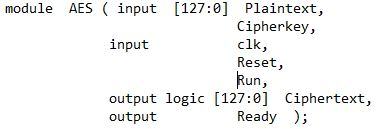
\includegraphics[width=0.45\textwidth]{AES.jpg}
	\label{fig:AES}
\end{figure}

The AES module is the main decryption algorithm implementation. It contains inputs of Reset and Run, along with 128-bits of encrypted text and 128-bits of a key. It outputs a 128-bit value containing the plaintext of the encrypted input after finishing. The main algorithm is explained in the lab manual, as well as below in the State Diagram section. \\

The module essentially loops through 10 rounds of calculations with each round containing the correct cycle of calculations as defined by the state machine. In order to avoid confusion, the rounds are looped backward from Round 9 to Round 0 in order to clearly show the decryption. \\

\textit{io\_module}\\
\vspace{-4mm}

\begin{figure}[h]
	\centering
	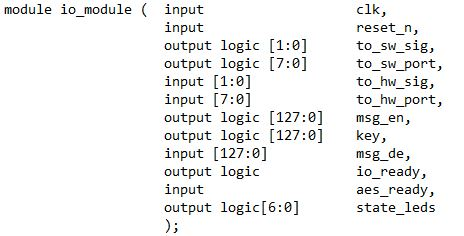
\includegraphics[width=0.45\textwidth]{iomodule.jpg}
	\label{fig:iomodule}
\end{figure}

The io\_module provides the communication between the hardware and software.  The module follows a very large state machine diagram shown in Figure \ref{fig:io-module}. Inputs include the decrypted message, hardware port and sig signals to control the movement of the message, clock, reset, and AES ready bit.  Outputs include 128-bit encrypted messaage and key, software port and sig signals,and an IO ready bit. \\

Io\_module must generate the proper acknowledgement signals to send to the software and process the correct acknowledgement signals from the software. As mentioned before, the module must utilize a state-machine to generate these proper bits and this is shown later on in the "State Diagram Section". \\

\textit{KeyExpansion}\\
\vspace{-4mm}

\begin{figure}[h]
	\centering
	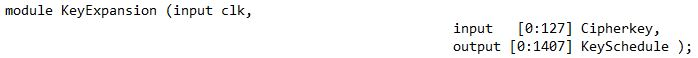
\includegraphics[width=0.45\textwidth]{KeyExpansion.jpg}
	\label{fig:KeyExpansion}
\end{figure}

The KeyExpansion module takes in the Cipher Key to create the first round key and then loops 10 more times creating 128-bit Round Keys each based off the previous key.  The 11 Round Keys are then stored into a 1408-bit Key Schedule. \\  

\textit{AddRoundKey}\\
\vspace{-4mm}

\begin{figure}[h]
	\centering
	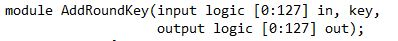
\includegraphics[width=0.45\textwidth]{AddRoundKey.jpg}
	\label{fig:AddRoundKey}
\end{figure}

The AddRoundKey module fetches a 4-word, 128-bit Round key from the pre-computed Key Schedule and bitwise XORs with the corresponding byte from the updating 128-bit state. The figure below shows a diagram of the AddRoundKey module. \\

\begin{figure}[h]
	\centering
	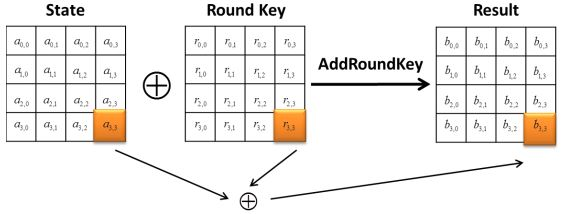
\includegraphics[width=0.45\textwidth]{AddRoundKeydia.jpg}
\end{figure}  


\textit{SubBytes,InvSubBytes}\\
\vspace{-4mm}

\begin{figure}[h]
	\centering
	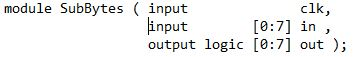
\includegraphics[width=0.45\textwidth]{SubBytes.jpg}
	\label{fig:SubBytes}
\end{figure}

SubBytes takes each byte of the updating state and transforms it by taking the multiplicative inverse of the Rijindael's finite field.  The transformation has been simplified into a black-box designated as the S-box (substitution box).  Inputs include the 256 byte array and clock.  Outputs include the transformed 256 byte array. The figure below portrays this module as a 4x4 matrix for sample.  \\

\begin{figure}[h]
	\centering
	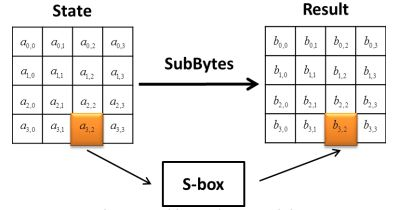
\includegraphics[width=0.45\textwidth]{SubBytesdia.jpg}
	\label{fig:SubBytesdia}
\end{figure}

The InvSubBytes module is similar to the SubBytes module except that the S-box is replaced by its inverse to reverse the encryption process.  \\

\textit{InvSubBytes\_16}\\
\vspace{-4mm}

\begin{figure}[h]
	\centering
	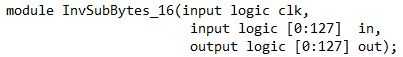
\includegraphics[width=0.45\textwidth]{InvSubBytes_16.jpg}
	\label{fig:InvSubBytes_16}
\end{figure}


InvSubBytes\_16 is a submodule of InvSubBytes.  It takes in the entire state during the InvSubBytes round and performs the appropriate substitution for each row and column. \\

\textit{ShiftRows,InvShiftRows}\\
\vspace{-4mm}

\begin{figure}[h]
	\centering
	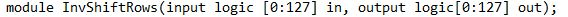
\includegraphics[width=0.45\textwidth]{InvShiftRows.jpg}
	\label{fig:InvShiftRows}
\end{figure}

The ShiftRows module takes in the 128-bit state and shifts the elements in each row n of the matrix by n-1 to the left.  The figure below shows a diagram of ShiftRows. \\ 

\begin{figure}[h]
	\centering
	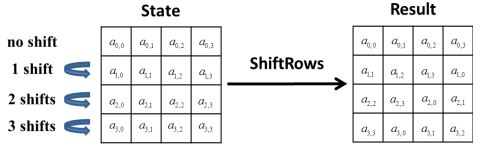
\includegraphics[width=0.45\textwidth]{ShiftRowsdia.jpg}
	\label{fig:InvShiftRows}
\end{figure}

The InvShiftRows module does exactly what The ShiftRows module does except it reverses the direction such the row n is right-circularly shifted by n-1 times. \\

\textit{MixColumns,InvMixColumns}\\
\vspace{-4mm}

\begin{figure}[h]
	\centering
	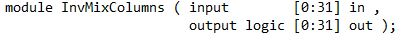
\includegraphics[width=0.45\textwidth]{InvMixColumns.jpg}
	\label{fig:InvMixColumns}
\end{figure}

The MixColumns module takes each of the four words from the state individually and goes through invertible linear tranformations over GF($2^8$) including multiplication by a fixed polynomial matrix to linearly combine the four bytes of each word to form a new Word.\\

\textit{HexDriver}\\
\vspace{-4mm}

This module contains the logic necessary to output values in binary/decimal in hex on the hex displays on board the Altera DE2-115.\\


%SECTION 4 - Description of USB Protocol & Changes
\section{Software/Hardware State Diagram}
The software/hardware state diagram is handled in io\_module and is shown in Figure \ref{fig:io-module}.

%SECTION 5 - State Diagram for Decryption 
\section{Decryption State Diagram}
The decryption state diagram is split up into two FSMs for simplicity. One is referred to as the Calculation FSM and the other is referred to as the Round FSM. There are a total of 10 rounds with an extra round to ensure the key\_expansion algorithm performs. Each round a series of calculations are performed as determined in the algorithm outlined in the description PDF of this lab. The Round FSM is shown in Figure \ref{fig:round-state} and the Calculation FSM is shown in Figure \ref{fig:calc-state}. Last, the AES Controller state machine is shown in Figure \ref{fig:AES_circuit}.

%SECTION 6 - Schematic/Block Diagram
\section{Schematic/Block Diagram}
The schematics and block diagram for the Top Level Module, the AES Controller, and AES Encryption Module can be found in "Figures Section".

%SECTION 7 - Annotated Pre-Lab Waveforms
\section{Annotated Pre-Lab Waveforms}
The annotated pre-lab waveforms can be found in Figure \ref{fig:0-500}, \ref{fig:500-1000}, \ref{fig:1000-1500}, and \ref{fig:1500-2000} for a 2000ns period. The ending decrypted value given plaintext of "daec3055df058e1c39e814ea76f6747e" with a key of "0102030405060708090a0b0c0d0e0f" is "ece298ece298...dc".

%SECTION 8 - Post Lab - 
\section{Post Lab}
\begin{table}[htbp]
	\centering
	\begin{tabular}{c|c}	% ccccccc indicates 7 center aligned columns
		\toprule	% top separator
		Resource & Value \\
		\midrule
		LUT & 5510\\
		DSP & 0\\
		Memory (BRAM) & 599,040\\
		Flip-Flop & 667\\
		Frequency &  141.88 MHz\\
		Static Power & 102.29 mW\\
		Dynamic Power & 0.77 mW\\
		Total Power & 187.27 mW\\
		\bottomrule	% bottom separator
	\end{tabular}%	
	\caption{Design Statistics}
	\label{tab:design}
\end{table}

\begin{enumerate}
	\item Which would you expect to be faster to complete encryption/decryption, the software or hardware? Is this what your results show?
	\begin{itemize}
	\item The faster encryption/decryption is expected to be the hardware because programming in software (specifically in C) is meant for generalized processors and thus must go through more clock cycles to do more compared to that of the hardware. The hardware is dedicated to the task at hand, and thus is faster. Specifically about 10 times as fast as the software as shown below by our metrics. \\
		
			\setlength{\leftskip}{24pt}Software Speed: 0.0058 MB/s \\
			Hardware Speed: 0.00043 MB/s (simulation)\\
			
	\end{itemize}
	\item If you wanted to speed up the hardware, what would you do? (Note: restrictions of this lab do not apply to answer this question)
	\begin{itemize}
		\item Instead of containing separate modules for each of the operations, these can be combined into a single module and the entire computation for one round can be done in a single state. This would significantly decrease the amount of time taken for one state to process. 
	\end{itemize}
\end{enumerate}


%SECTION 9 - Conclusion
\section{Conclusion}
Overall, this lab proved to be very difficult from both a hardware and software perspective. Programming the encryption algorithm in C was difficult for many reasons. Working with multidimensional arrays is never an easy task in C, and this lab seemed to put this skill to the test. The notation used throughout the algorithm is difficult to understand fully what should be passed into certain functions. However, once a basic working model of the encryption algorithm was developed, it was optimized for patterns, and condensed and therefore much easier to understand. \\

The hardware decryption was just as difficult as the software, if not more difficult. The finite state machines that were developed took a large amount of time to debug using ModelSim. The io\_module used to pass information to/from the software proved to be a large time-sink in and of itself. \\

In the end, the team did not receive full points for demo due to a glitch in passing the data to/from software. However, partial credit was received for showing simulations.\\

Overall this lab was one of the most difficult ECE385 labs, however it was one of the most rewarding to understand in the end. AES encryption/decryption is now very clear to the team.

\clearpage
\onecolumn
%SECTION 10: Figures
\section{Figures}


\begin{figure} [H]
	\centering
	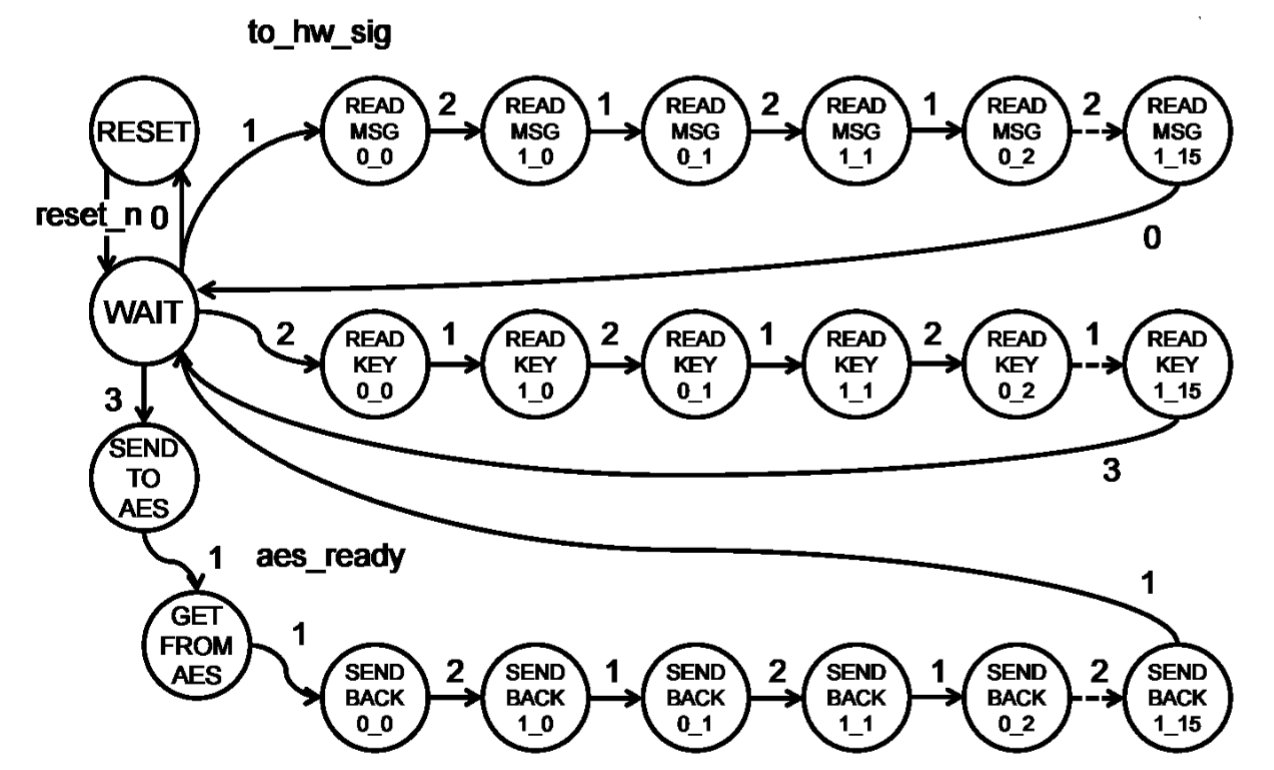
\includegraphics[scale=.6]{IO_Module_State_Diagram.png}
	\caption{IO Module Hardware/Software State Diagram\label{fig:io-module}}
\end{figure}  


\begin{figure} [H]
	\centering
	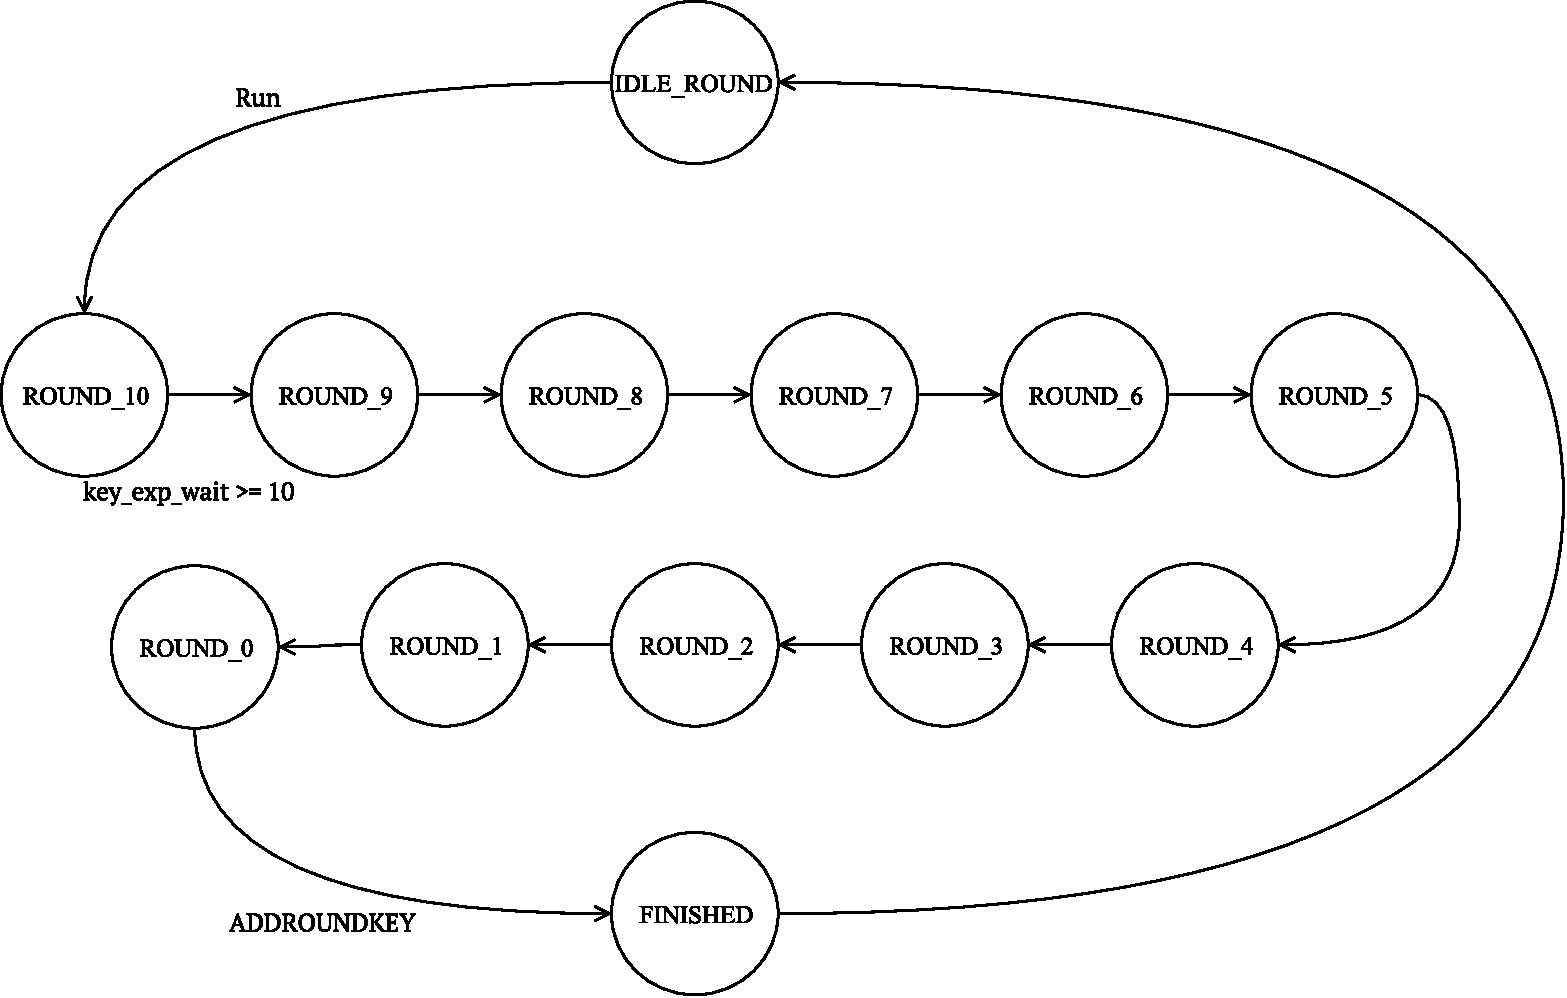
\includegraphics[scale=.6]{Decryption_Round_State_Diagram.pdf}
	\caption{Decryption Round State Diagram\label{fig:round-state}}
\end{figure}          

\begin{figure} [H]
	\centering
	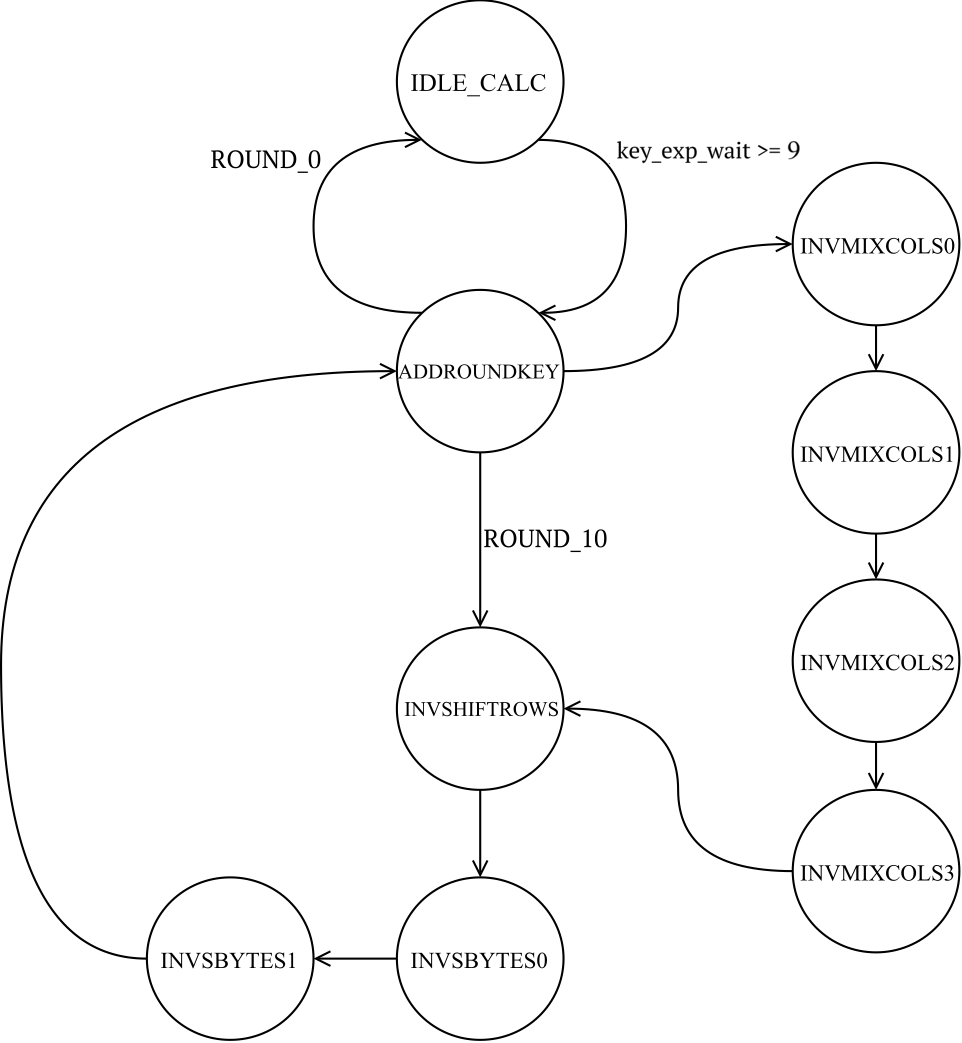
\includegraphics[scale=.6]{Calc_State_Diagram.png}
	\caption{Calculation State Diagram\label{fig:calc-state}}
\end{figure}         


\begin{figure} [H]
	\centering
	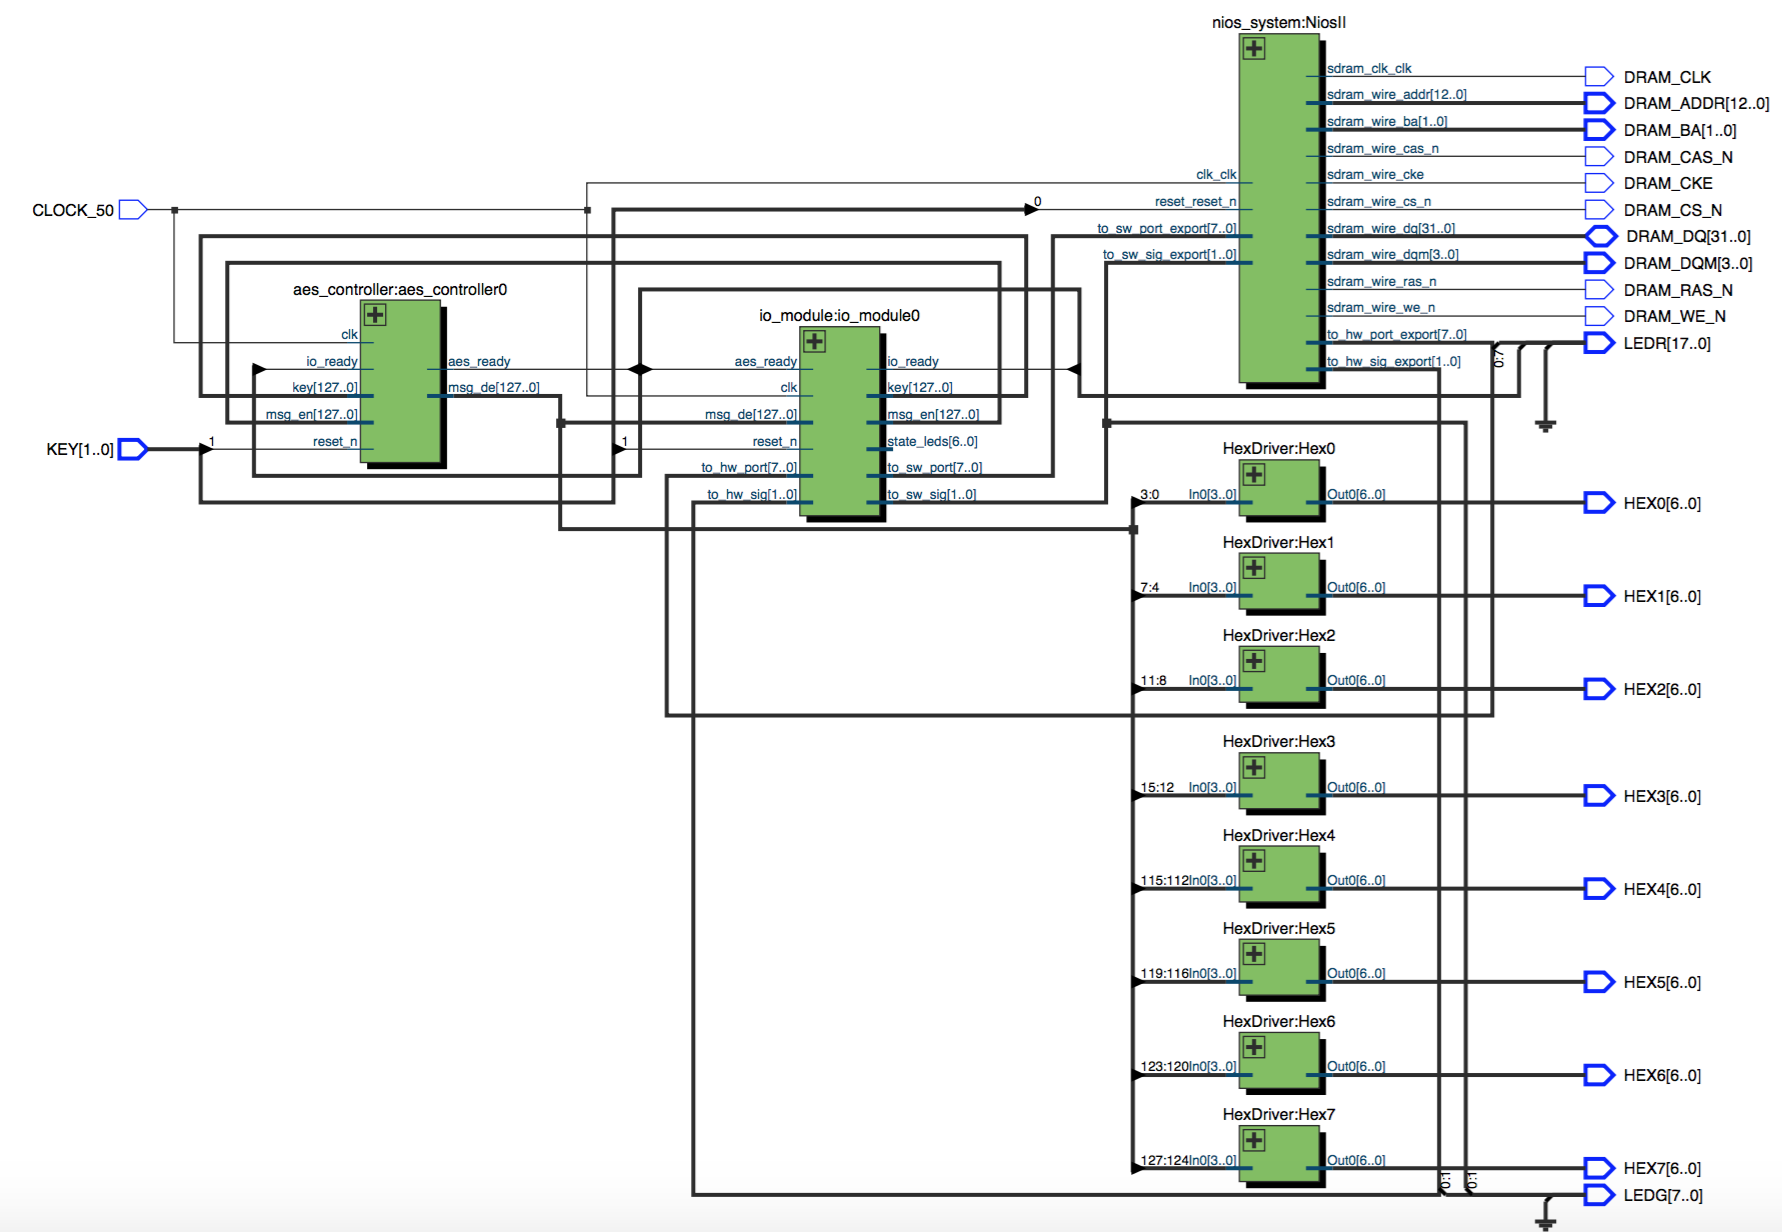
\includegraphics[scale=.5]{top_level_circuit.png}
	\caption{Top Level Circuit Diagram\label{fig:top-level-circuit}}
\end{figure}   

\begin{figure} [H]
	\centering
	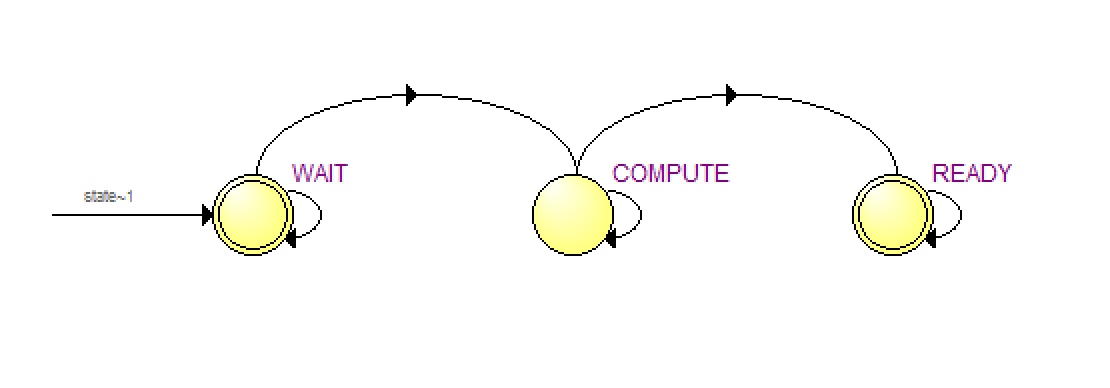
\includegraphics[scale=.5]{AES_controller_state.png}
	\caption{AES Controller State Diagram\label{fig:aes-cont-state}}
\end{figure}    

\begin{figure} [H]
	\centering
	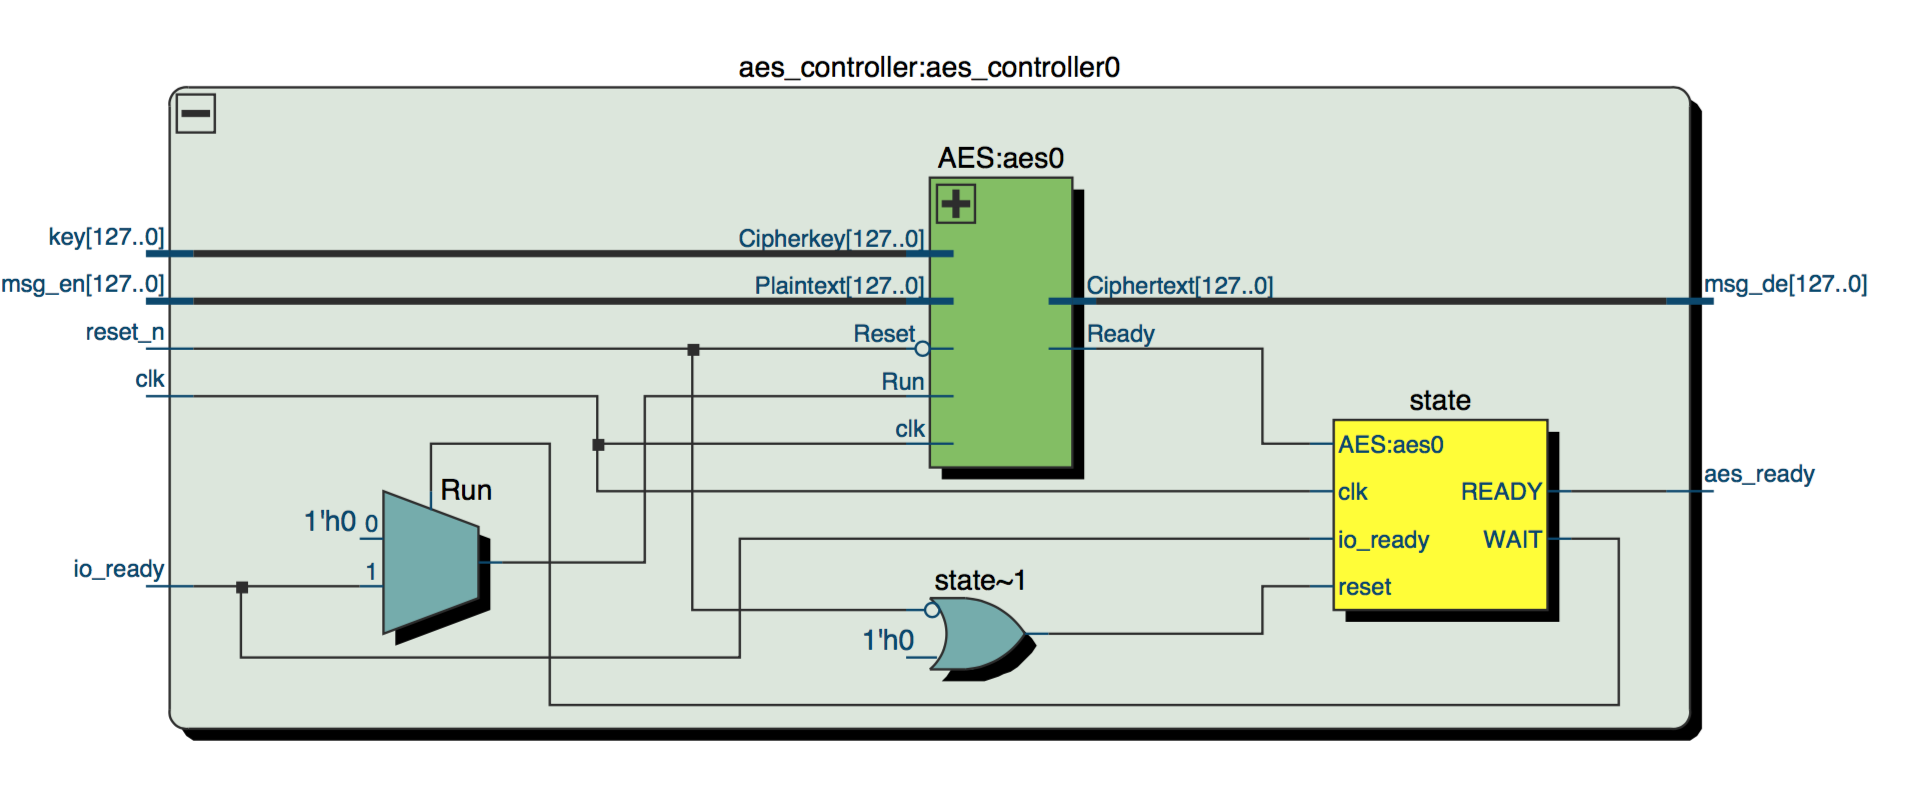
\includegraphics[scale=.5]{aes_controller_circuit.png}
	\caption{AES Controller Circuit\label{fig:aes_cont_circuit}}
\end{figure}    

\begin{figure} [H]
	\centering
	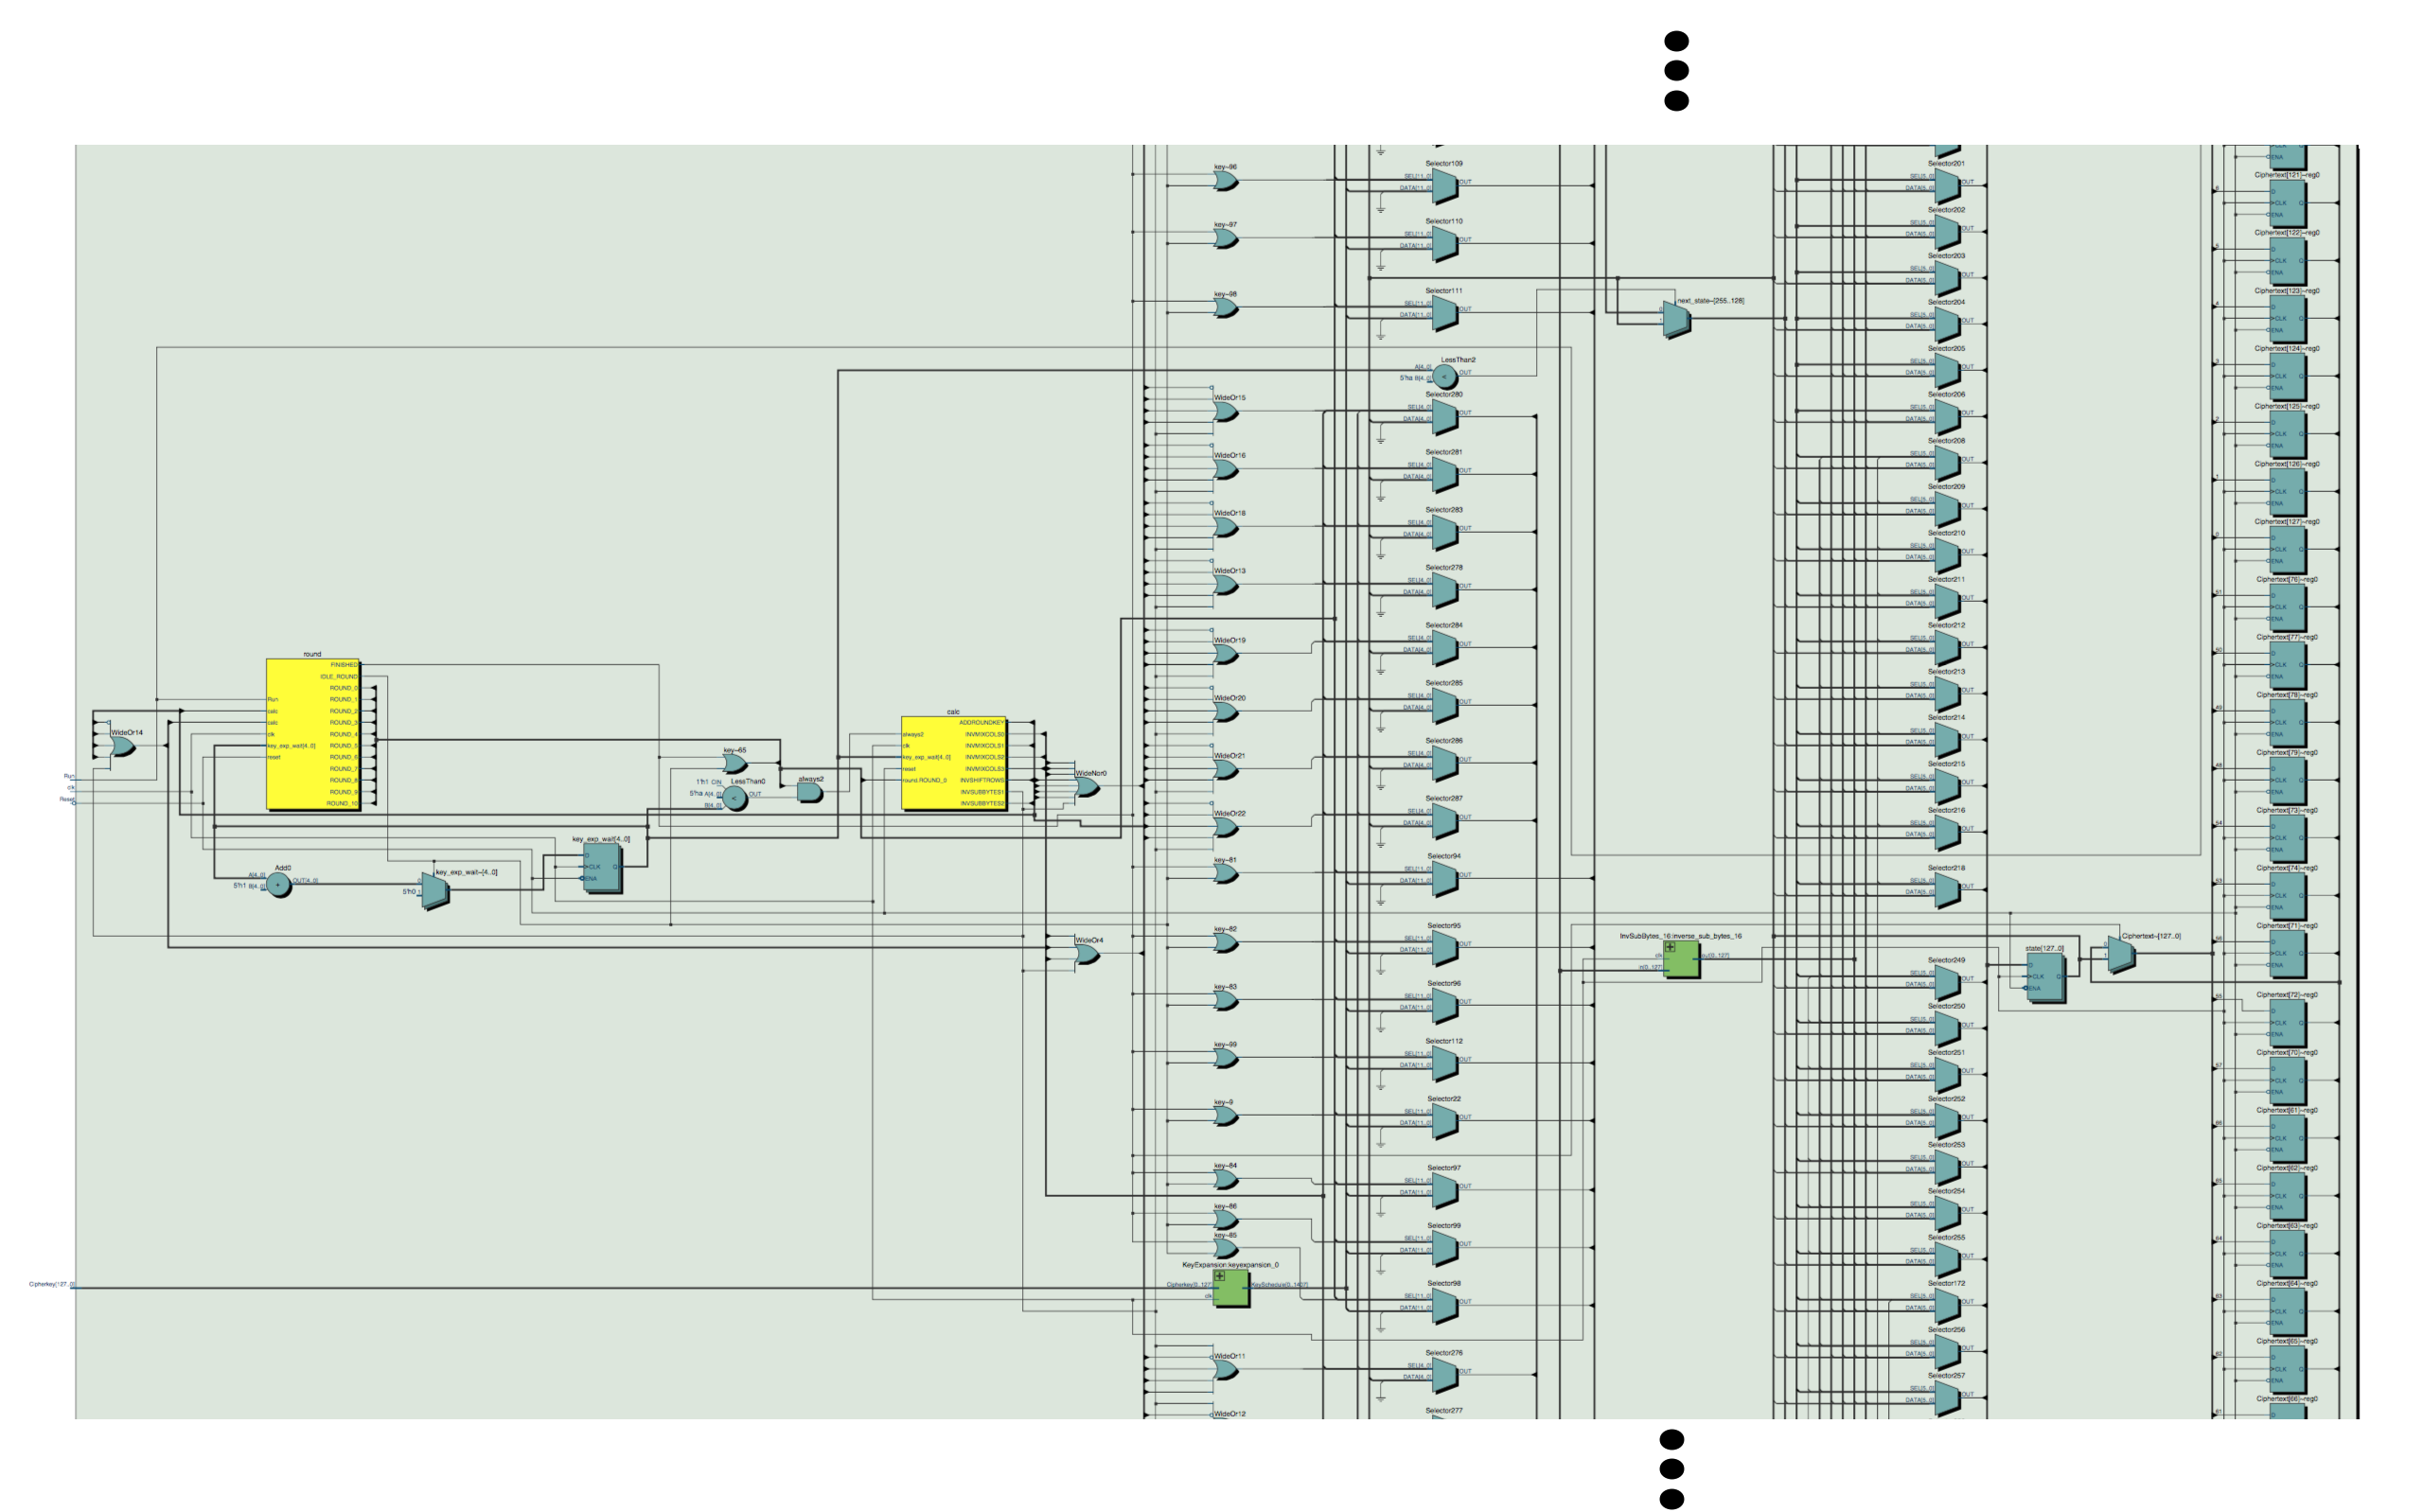
\includegraphics[scale=.35]{AES_circuit.png}
	\caption{AES Circuit\label{fig:AES_circuit}}
\end{figure}    


\begin{figure} [H]
	\centering
	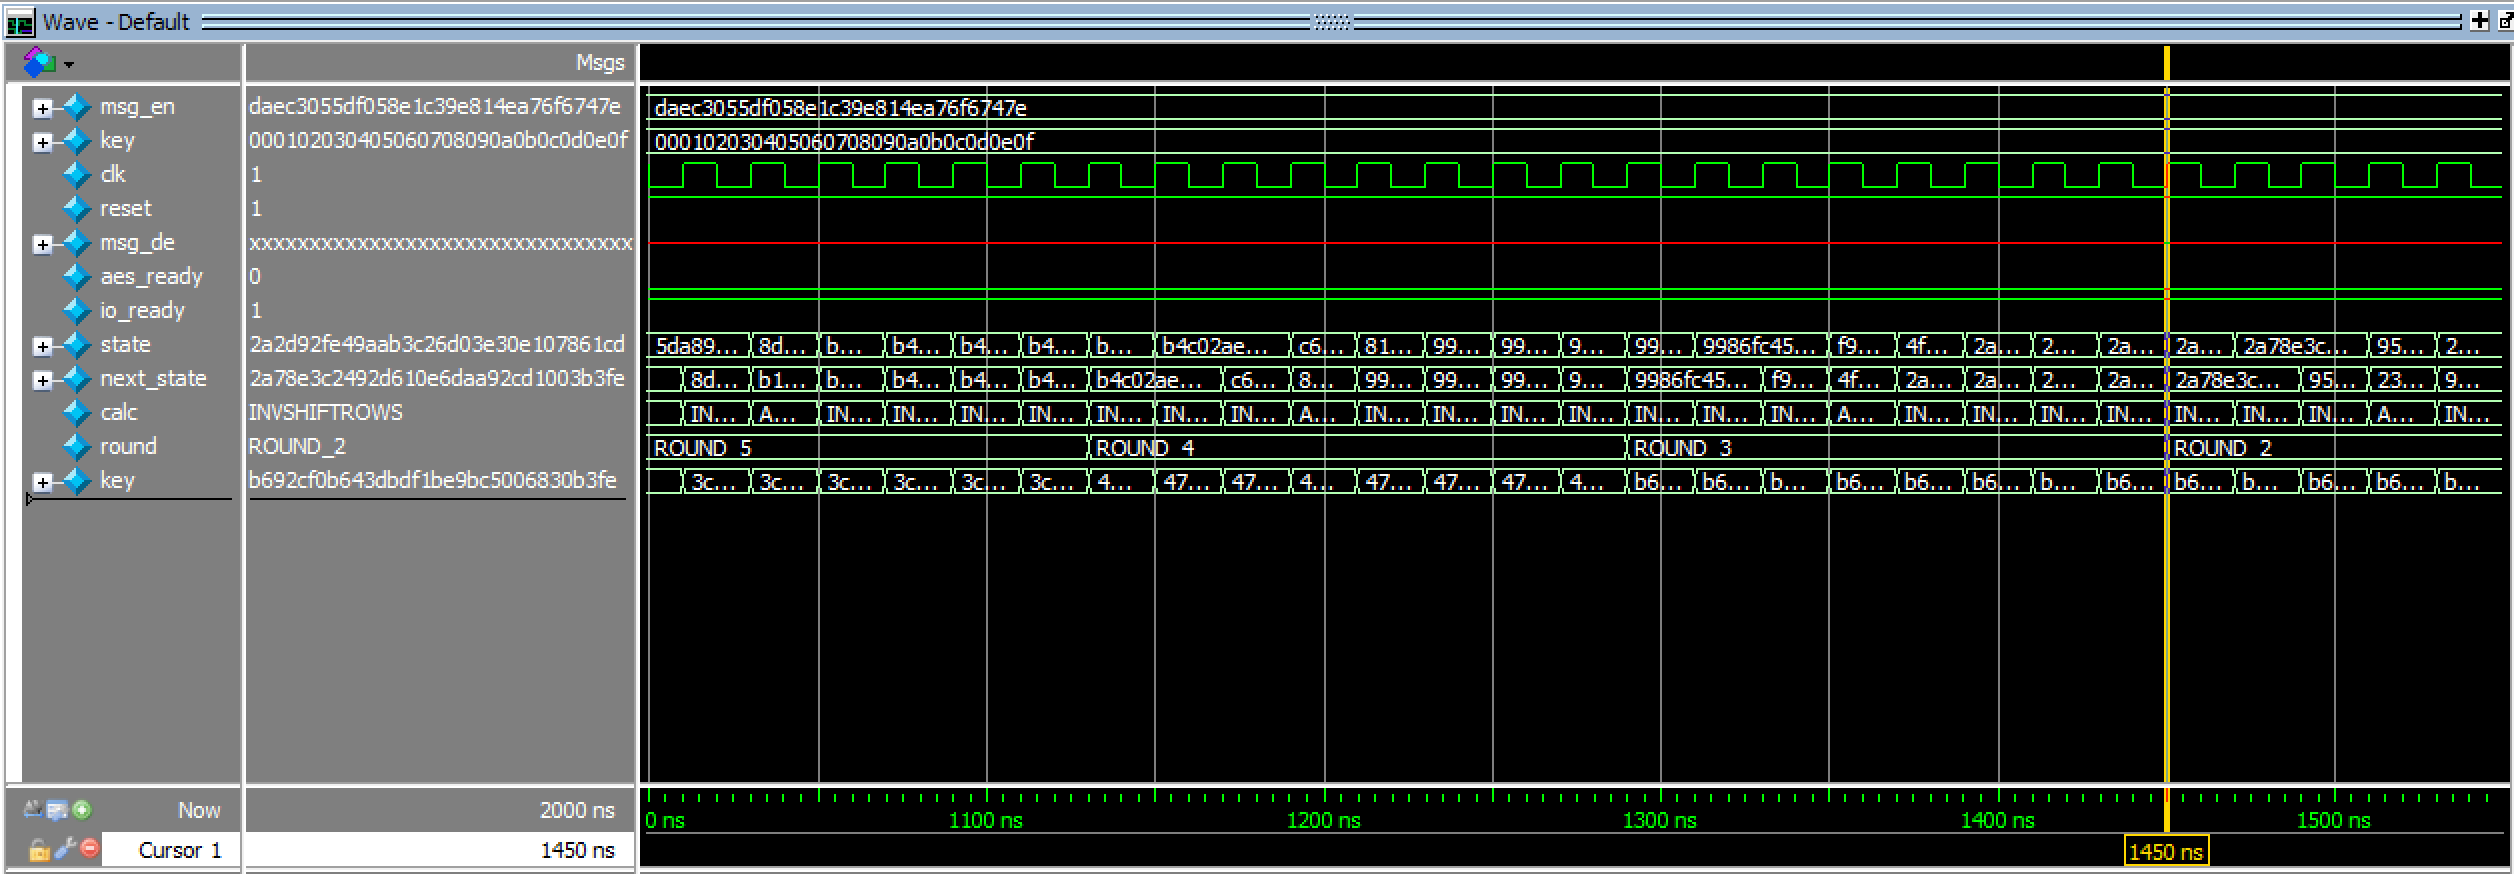
\includegraphics[scale=.35]{simulate-0-500.png}
	\caption{Simulation 0 - 500ns\label{fig:0-500}}
\end{figure}          


\begin{figure} [H]
	\centering
	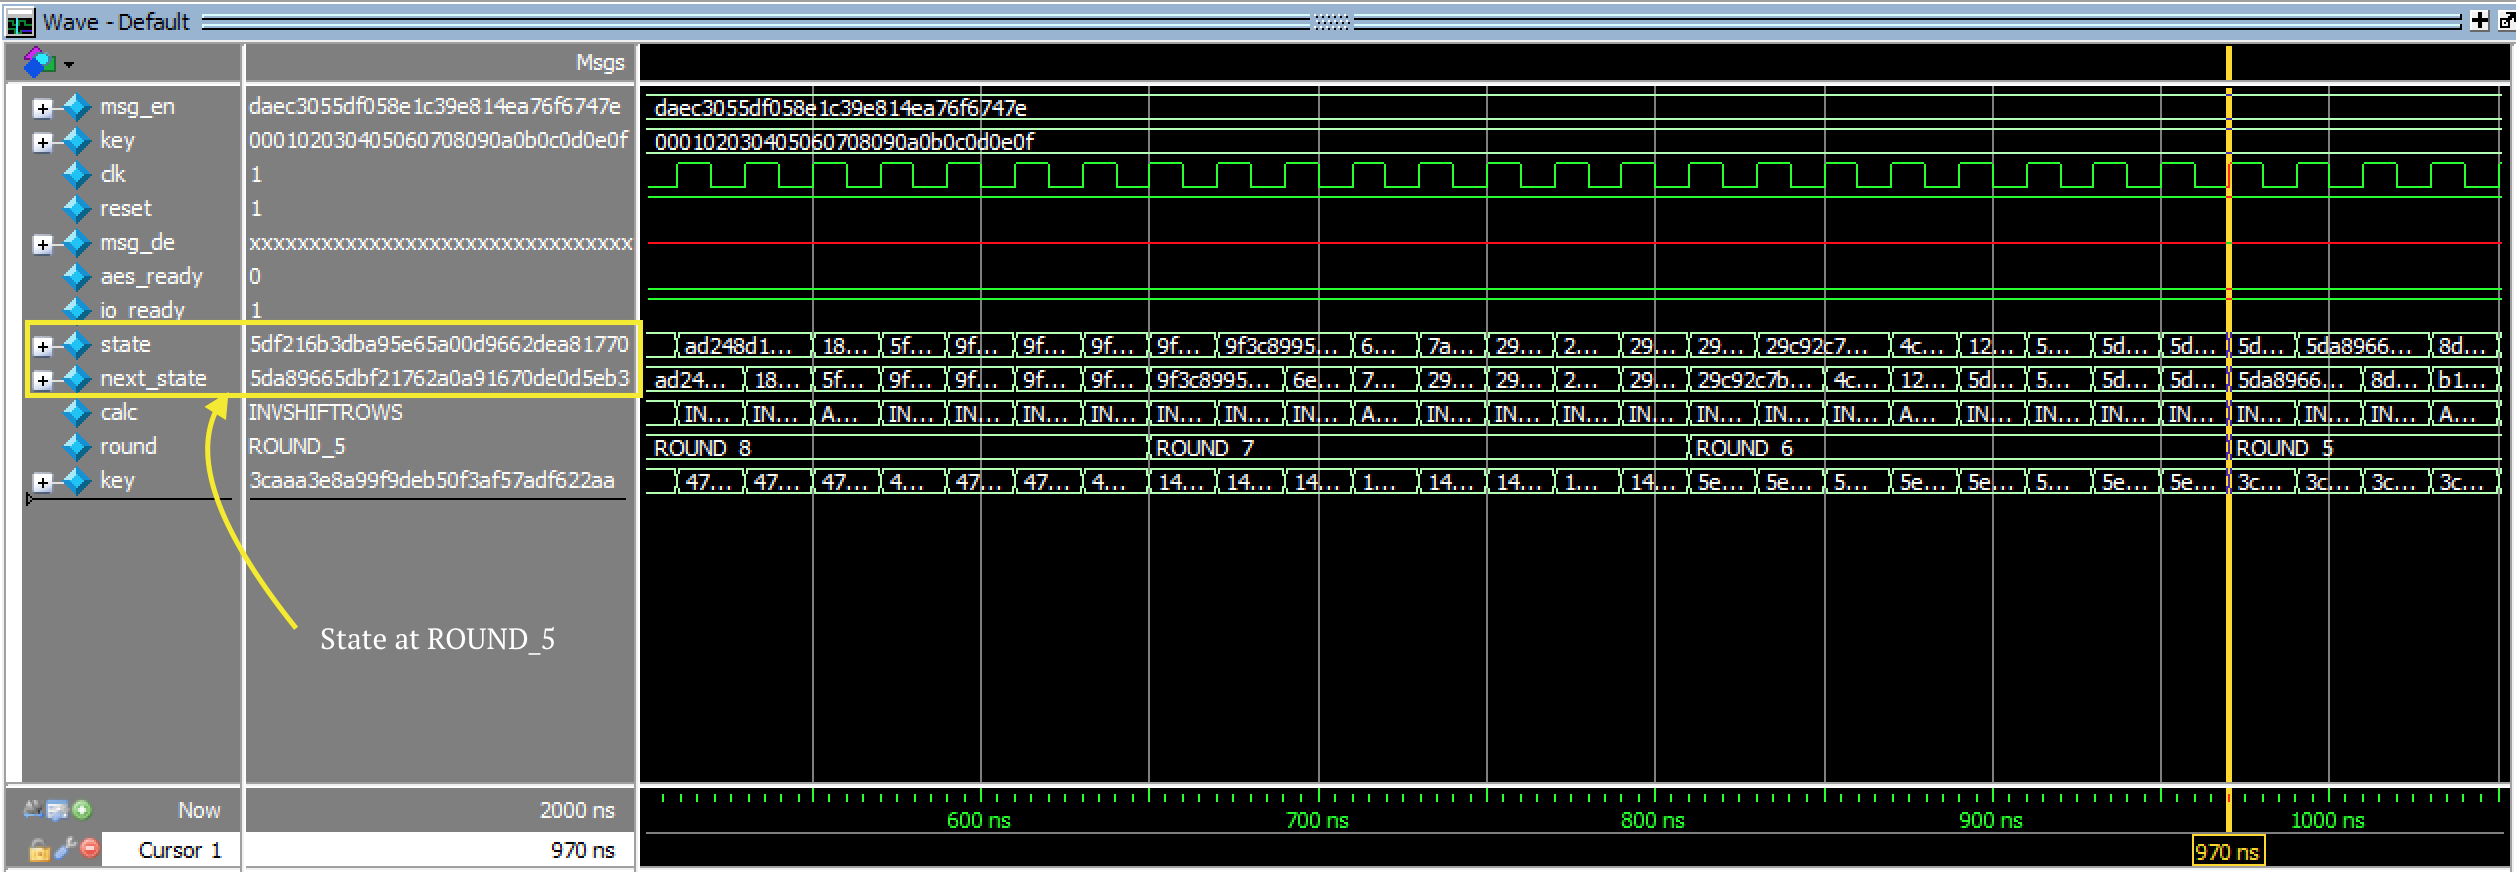
\includegraphics[scale=.35]{simulate-500-1000.png}
	\caption{Simulation 500 - 1000ns\label{fig:500-1000}}
\end{figure}          


\begin{figure} [H]
	\centering
	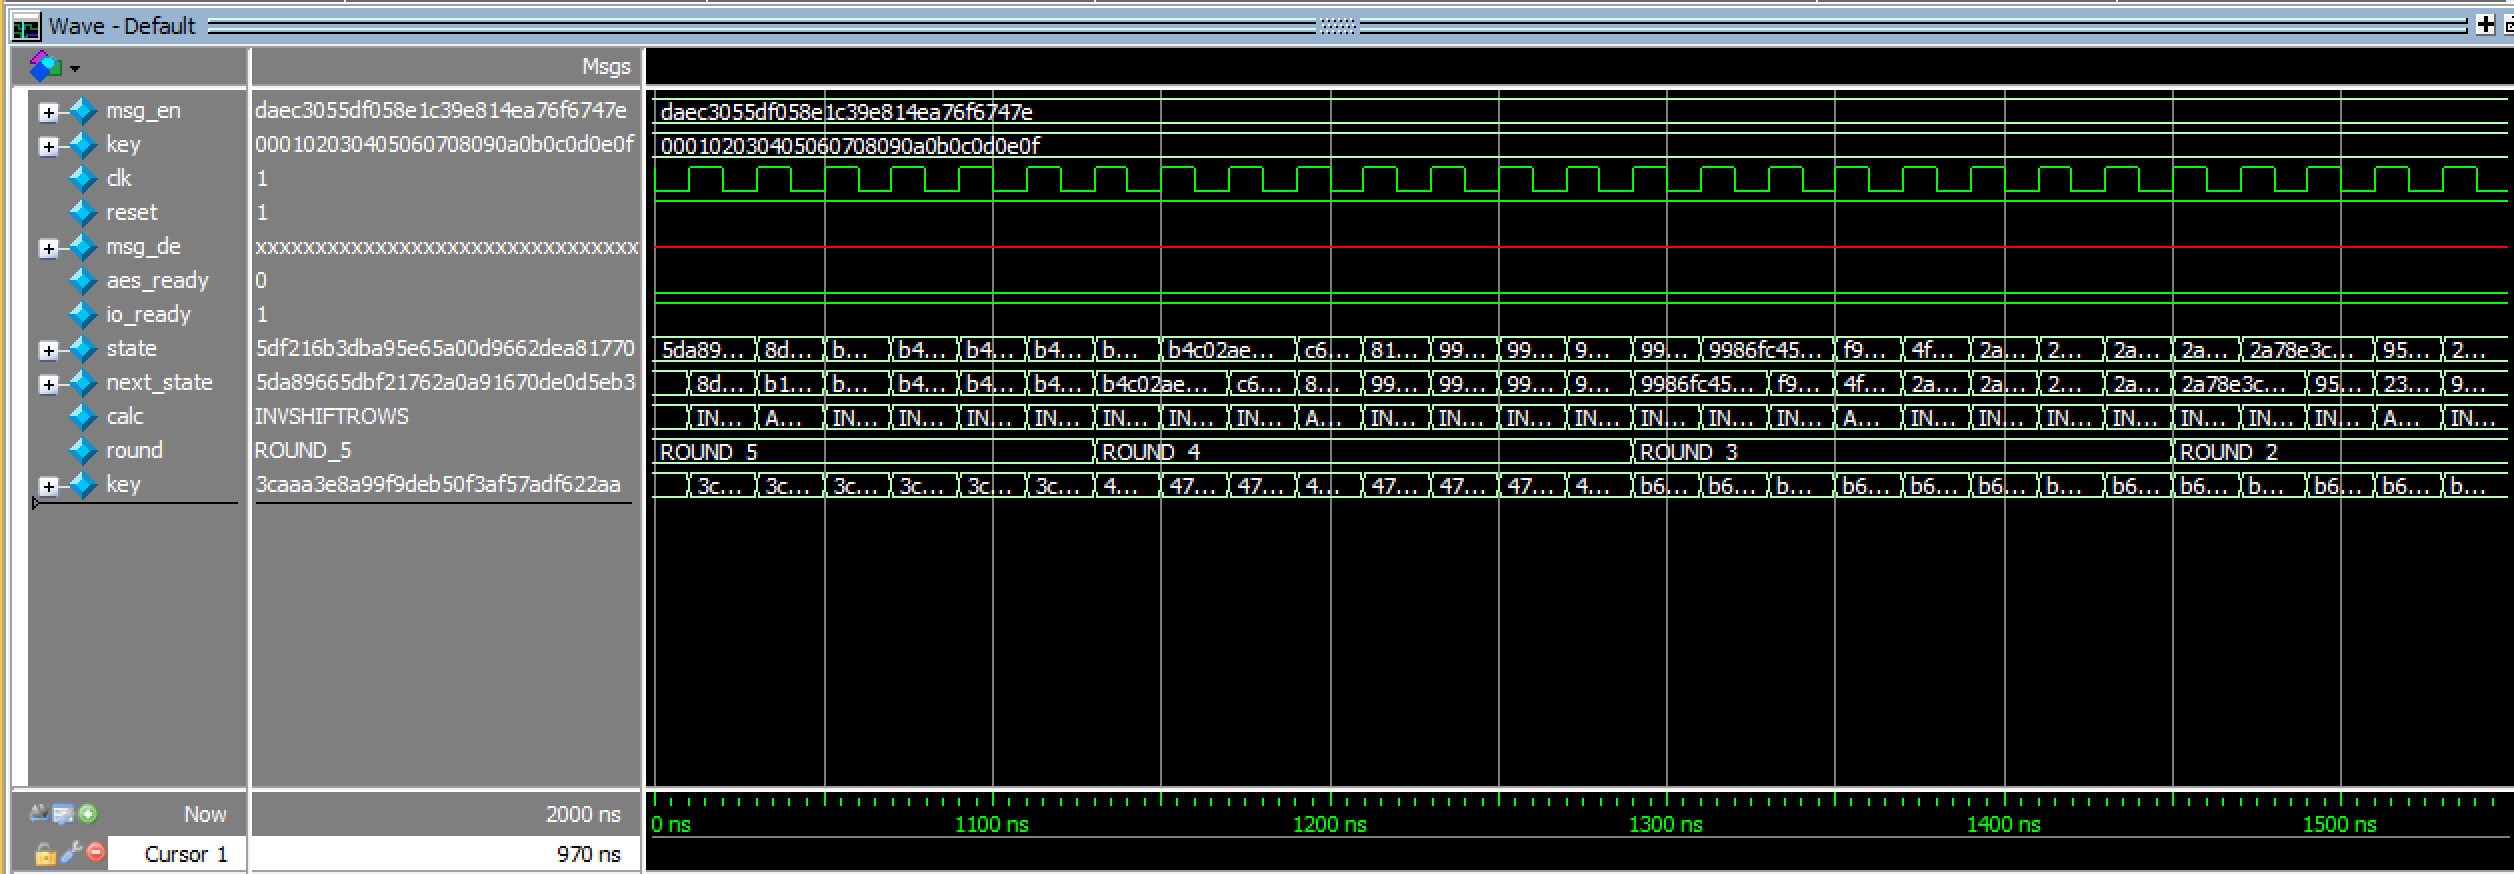
\includegraphics[scale=.35]{simulate-1000-1500.png}
	\caption{Simulation 1000 - 1500ns\label{fig:1000-1500}}
\end{figure}          


\begin{figure} [H]
	\centering
	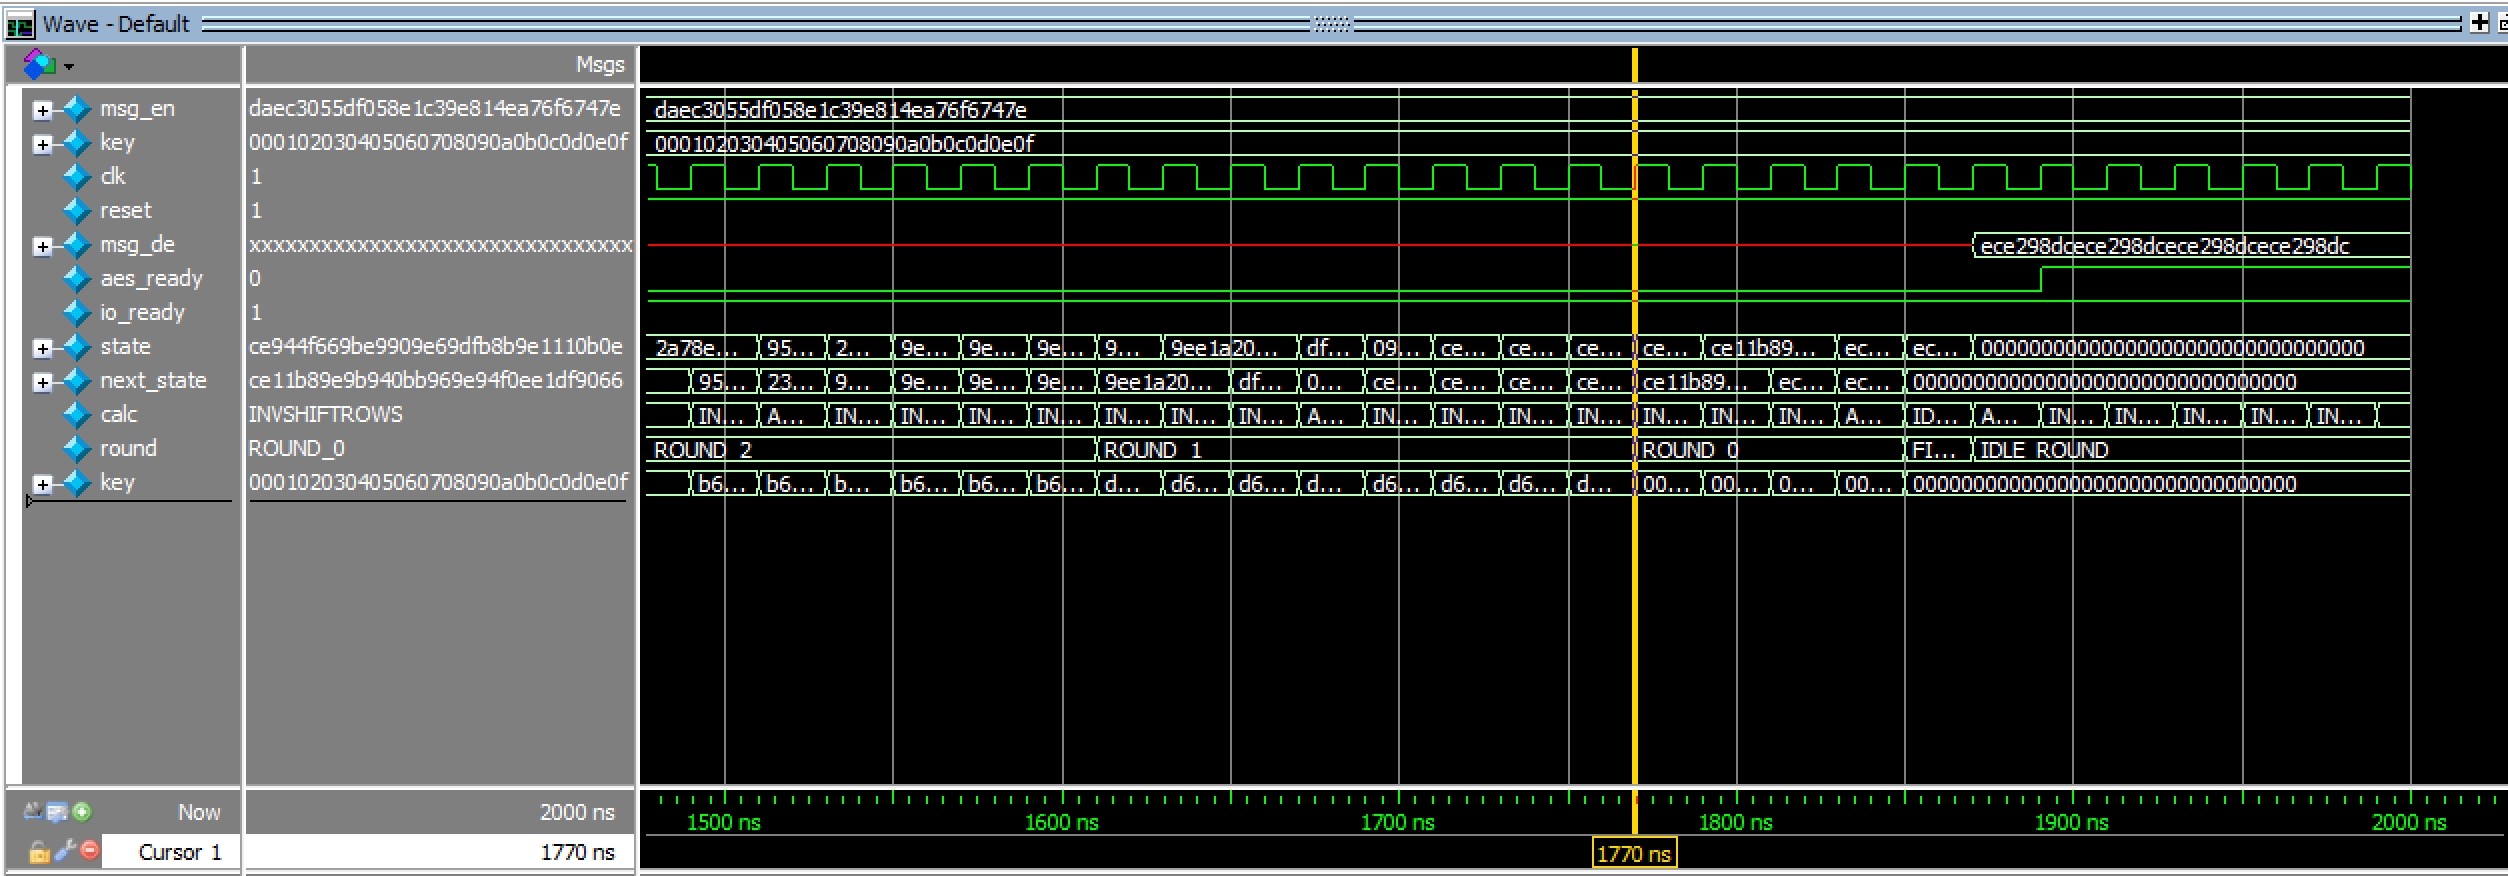
\includegraphics[scale=.35]{simulate-1500-2000.png}
	\caption{Simulation 1500-2000ns\label{fig:1500-2000}}
\end{figure}          



\end{document}
